%\documentclass[11pt]{beamer}
\documentclass[11pt,handout,aspectratio=1610]{beamer}

\usepackage[utf8]{inputenc}
\usepackage[T1]{fontenc}
\usepackage[spanish]{babel}
\usepackage{latexsym} 
\usepackage{amsmath}
\usepackage{amsfonts}
\usepackage{amssymb}
\usepackage{esint}
\usepackage{array}
\usepackage{multirow}
\usepackage{xcolor}
\usepackage{graphicx}
\usepackage{tikz}
\usepackage{tikz-3dplot}
\usetikzlibrary{babel}
\usetikzlibrary{calc,patterns,decorations.pathmorphing,decorations.markings}
\usetikzlibrary{arrows.meta} % for arrow size
\tikzset{>=latex} % for LaTeX arrow head
\usepackage{xcolor}
\usepackage{epstopdf}
\usepackage[nointegrals]{wasysym}
\usepackage{hyperref}
\usepackage{cancel}
\usepackage[font=small,labelfont={small,bf},margin=0.5cm,justification=justified]{caption}
\usepackage[font=small,labelfont={small,bf}]{subcaption}

\usetheme{Berkeley}
\usecolortheme{seahorse}
\uselanguage{Spanish}

\newcommand{\sgn}{\mathop{\text{sgn}}}
\newcommand{\diff}[0]{\text{d}}
\newcommand{\fdiff}[2]{\dfrac{\text{d} #1}{\text{d} #2}}
\newcommand{\pdiff}[2]{\frac{\partial #1}{\partial #2}}
\newcommand{\pddiff}[2]{\frac{\partial^2 #1}{\partial #2^2}}
\newcommand{\fddiff}[2]{\frac{\diff^2 #1}{\diff #2^2}}
\newcommand{\grado}[0]{^{\circ}}
\newcommand{\chel}[4]{^{#1}_{#2}\text{#3}^{#4}}
\newcommand{\valmed}[1]{\left\langle #1 \right\rangle}
\newcommand{\E}[1]{\times 10^{#1}}
\newcommand{\ver}[1]{\hat{\mathbf{#1}}}
\newcommand{\vecg}[1]{\boldsymbol{#1}}
\newcommand{\iu}{\text{i}}
\newcommand{\norm}[1]{\left\vert\left\vert #1 \right\vert\right\vert}
\newcommand{\abs}[1]{\left\vert #1 \right\vert}
\newcommand{\tens}[1]{\mathbb{#1}}
\newcommand{\rr}{\mathbb{R}}
\newcommand{\zz}{\mathbb{Z}}
\newcommand{\nn}{\mathbb{N}}
\newcommand{\logoUNAHUR}{
\includegraphics[scale=0.15]{/home/shluna/Proyectos/Clases_Fisica_III/imgs/logo-universidad-nacional-de-hurlingham_preview_rev_1.png}}
\newcommand{\vs}{\vspace{11pt}}
\newcommand{\un}[1]{\text{#1}}

\title{Fenómenos ondulatorios}
\subtitle{Unidad 4}
\author{Física III}
\institute{Instituto de Tecnología e Ingeniería \\ \vspace{0.25cm} Universidad Nacional de Hurlingham}
\date{ }
\logo{\logoUNAHUR}

\AtBeginSection[]{
  \begin{frame}
  \vfill
  \centering
  \begin{beamercolorbox}[sep=8pt,center,shadow=true,rounded=true]{title}
    \usebeamerfont{title}\insertsectionhead\par%
  \end{beamercolorbox}
  \vfill
  \end{frame}
}

\tdplotsetmaincoords{70}{110}

\begin{document}

\frame{\titlepage}

\begin{frame}{En esta clase veremos:}
    \tableofcontents
\end{frame}

\section{Introducción}

\begin{frame}{Introducción}

    Una de las características más interesantes de los medios capaces de deformarse es la de transmitir ondas de un punto a otro dentro de su extensión, tal como ocurre cuando se arroja una pequeña piedra a una masa de agua estancada.

    \vs

    La presente unidad tiene como propósito estudiar el fenómeno de la transmisión de las ondas en el espacio, pero para ello debemos definir algunos conceptos.

    \begin{block}{Definición}
        Una \emph{onda} es una perturbación o señal, generada por un \emph{emisor} que se propaga a través de un \emph{medio} y, eventualmente, llega hasta un \emph{receptor}.  
    \end{block}

    Podemos notar en esta definición que para generar, transmitir y detectar una onda son necesarios un emisor, un medio y un receptor, respectivamente.

\end{frame}

\begin{frame}
    \frametitle{Tipos de onda}

    Las ondas pueden clasificarse según el medio en el que se propaguen. Tres ejemplos importantes son las siguientes:
    \begin{itemize}
        \item \textbf{Ondas mecánicas}: Son aquellas que se propagan a través de un medio material, como por ejemplo en un sólido deformable (\emph{ondas elásticas}) y en un fluido (\emph{olas}, \emph{ondas de presión}, \emph{sonido}).
        \item \textbf{Ondas elétromagnéticas}: Como su nombre lo sugiere, son las que se propagan a través del campo electromagnético, tales como la luz visible, ultravioleta, rayos X, rayos gamma, infrarrojo, etc.
        \item \textbf{Ondas gravitacionales}: Aquellas que se propagan a través del campo gravitatorio.
    \end{itemize}

\end{frame}

\section{Descripción matemática de las ondas}

\begin{frame}{Descripción matemática de las ondas}

    Anteriormente señalamos que una onda es una perturbación que se propaga por un determinado medio. Entendemos por perturbación a toda modificación o apartamiento del estado de equilibro, por lo tanto, es de fundamental importancia identificar las variables que definen el estado de equilibrio de un sistema dado. A modo de ejemplo, consideremos una cuerda tensa que se encuentra de forma horizontal sujeta a dos soportes, tal como se muestra en la Figura~\ref{fig:cuerda_equilibrio}.

    \vs 
    \begin{figure}
        \centering
        
\includegraphics[width=0.6\textwidth]{../figs/cuerda_equilibrio.pdf}
        \caption{Cuerda tensa en equilibrio.}
        \label{fig:cuerda_equilibrio}
    \end{figure}

    Supongamos ahora que en el instante $t_0$ se le da a la cuerda un impulso tal que la cuerda se genera una perturbación que se propaga hacia la derecha con cierta rapidez $v$, como la que se muestra a continuación.

\end{frame}

\begin{frame}{Descripción matemática de las ondas}

    Supongamos ahora que en cierto instante se le da a la cuerda un impulso tal se genera una perturbación que se propaga hacia la derecha con cierta rapidez $v$, como la que se muestra a continuación.

    \begin{figure}
        \centering
        \begin{tikzpicture}[scale=1]
            \def\Px{1.8}

            \draw[->,thick] (-0.5,0) -- (5,0) node[below]{$x$};
            \draw[->,thick] (0,-0.5) -- (0,2) node[left]{$y$};
            \draw[blue,very thick,samples=100,smooth,variable=\x,domain=0:4.5] plot(\x,{1.25*exp(-(\x-2)^2/0.5)});

            \draw[thick,red,->] (2,1.5) -- node[above,midway]{$\vec{v}$} (3,1.5); 
            
            \coordinate (P) at (\Px,{1.25*exp(-(\Px-2)^2/0.5)});
            \coordinate (Px) at (\Px,0);
            
            \fill[black] (P) circle (0.5mm);
            \fill[black] (Px) circle (0.5mm);
            
            \draw[<->] (Px) -- node[right,midway]{$y$} (P);
        \end{tikzpicture}
    \end{figure}

    En este caso, la perturbación se describe como la distancia $y$ (hacia arriba o hacia abajo) en la que la cuerda se aparta de la línea horizontal que caracteriza su estado de equilibrio.

    \vs

    La coordenada $y$ de cada punto de la cuerda debe ser una función tanto de su posición $x$ como del tiempo $t$, esto es: $y = f(x,t)$. 

\end{frame}

\begin{frame}{Descripción matemática de las ondas}

    Puede comprobarse que, en la medida que puedan despreciarse todos los efectos disipativos, la forma del pulso se conserva a lo largo de todo su recorrido por la cuerda y que este se propaga a velocidad constante.

    \vs 

    Si $y = f(x,t_0)$ representa la forma del pulso en el instante $t_0$, en un instante de tiempo arbitrario $t$ posterior o anterior, el pulso se desplaza $s$ unidades hacia la derecha o hacia la izquierda, respectivamente, donde $$ s(t) = x_0 + v \left(t - t_0\right), $$ donde $x_0$ es el valor de $s$ en $t_0$, y, por lo tanto, en el instante $t$ la forma del pulso está dada por $y = f(x-s(t))$. En virtud de que la dependencia temporal está incluida en la expresión de $s(t)$, no es necesario incluirla en la forma $f(x-s(t),t)$.
 
\end{frame}

\begin{frame}{Descripción matemática de las ondas}
    
    Por otro lado, si la forma del pulso ha de conservarse, entonces la altura $y$ de un punto cuya abscisa es $x_1$, en cierto instante $t_1$, al cabo de cierto intervalo de tiempo $\Delta t$, la altura de otro punto de abscisa $x_2 = x_1 + v \, \Delta t$ debe ser también $y$ en el instante $t_2 = t_1 + \Delta t$, esto es: $$ y(x_2,t_2) = y(x_1,t_1) $$  

    \begin{figure}
        \centering
        \begin{tikzpicture}[scale=1]
            \def\Px{1.8}
            \def\Qx{6.8}

            \draw[->,thick] (-0.5,0) -- (10,0) node[below]{$x$};
            \draw[->,thick] (0,-0.5) -- (0,2) node[left]{$y$};
            \draw[blue,very thick,samples=100,smooth,variable=\x,domain=0:5,dashed] plot(\x,{1.25*exp(-(\x-2)^2/0.5)});
            \draw[blue,very thick,samples=100,smooth,variable=\x,domain=0:9.5] plot(\x,{1.25*exp(-(\x-7)^2/0.5)});

            \draw[thick,red,->] (2,1.5) -- node[above,midway]{$\vec{v}$} (3,1.5); 
            \draw[thick,red,->] (7,1.5) -- node[above,midway]{$\vec{v}$} (8,1.5); 
            
            \coordinate (P) at (\Px,{1.25*exp(-(\Px-2)^2/0.5)});
            \coordinate (Px) at (\Px,0);
            
            \fill[black] (P) circle (0.5mm);
            \fill[black] (Px) circle (0.5mm) node[below left]{$x_1$};
            
            \draw[<->] (Px) -- node[right,midway]{$y$} (P);

            \coordinate (Q) at (\Qx,{1.25*exp(-(\Qx-7)^2/0.5)});
            \coordinate (Qx) at (\Qx,0);
            
            \fill[black] (Q) circle (0.5mm);
            \fill[black] (Qx) circle (0.5mm) node[below right]{$x_2$};
            
            \draw[<->] (Qx) -- node[right,midway]{$y$} (Q);

            \draw[<->] (\Px,-0.5) -- node[fill=white]{$v \, \Delta t$} (\Qx,-0.5);
            \draw (\Px,-0.1) -- (\Px,-0.7);
            \draw (\Qx,-0.1) -- (\Qx,-0.7);
        \end{tikzpicture}
    \end{figure}
     
\end{frame}

\begin{frame}{Descripción matemática de las ondas}

    Puede demostrarse fácilmente que la condición $ y(x_2,t_2) = y(x_1,t_1) $ queda satisfecha si la perturbación está dada por $y(x,t) = f(x-s(t))$.

    \vs

    En conclusión, si la magnitud $\xi$ representa una desviación de cierto estado de equilibrio, entonces la propagación de esta perturbación se describe matemáticamente con una función $\xi = f(\vec{r}-\vec{s}(t))$, donde $\vec{r}$ es el vector de posición del punto genérico en el que se evalúa la perturbación y $\vec{s}(t)$ es una función vectorial lineal en el tiempo que describe el desplazamiento de la perturbación. 
    
    \vs

    Toda función que represente una onda se la suele llamar \emph{función de onda}.
     
\end{frame}

\begin{frame}{Descripción matemática de las ondas}

    En virtud de que la función de onda depende tanto de las coordenadas espaciales como del tiempo, podemos analizar la propagación de la perturbación asociada en el tiempo de forma análoga a como lo hicimos para el espacio.

    \vs

    Si ahora $y = f(x_0,t)$ representa la forma del pulso en función del tiempo, esto es cómo cambia la altura $y$ de un punto de la cuerda cuya abscisa es $x_0$ en el tiempo, entonces un \emph{desplazamiento} en el tiempo de esta función está dado por $y = f(t - \tau(x))$ donde, $$ \tau (x) = t_0 + \frac{x-x_0}{v} $$

    \begin{figure}
        \centering
        \begin{tikzpicture}[scale=1]
            \def\Px{1.8}
            \def\Qx{6.8}

            \draw[->,thick] (-0.5,0) -- (10,0) node[below]{$t$};
            \draw[->,thick] (0,-0.5) -- (0,2) node[left]{$y$};
            \draw[blue,very thick,samples=100,smooth,variable=\x,domain=0:5,dashed] plot(\x,{1.25*exp(-(\x-2)^2/0.5)});
            \draw[blue,very thick,samples=100,smooth,variable=\x,domain=0:9.5] plot(\x,{1.25*exp(-(\x-7)^2/0.5)});

            \draw[thick,red,->] (2,1.5) -- node[above,midway]{$\vec{v}$} (3,1.5); 
            \draw[thick,red,->] (7,1.5) -- node[above,midway]{$\vec{v}$} (8,1.5); 
            
            \coordinate (P) at (\Px,{1.25*exp(-(\Px-2)^2/0.5)});
            \coordinate (Px) at (\Px,0);
            
            \fill[black] (P) circle (0.5mm);
            \fill[black] (Px) circle (0.5mm) node[below left]{$t_1$};
            
            \draw[<->] (Px) -- node[right,midway]{$y$} (P);

            \coordinate (Q) at (\Qx,{1.25*exp(-(\Qx-7)^2/0.5)});
            \coordinate (Qx) at (\Qx,0);
            
            \fill[black] (Q) circle (0.5mm);
            \fill[black] (Qx) circle (0.5mm) node[below right]{$t_2$};
            
            \draw[<->] (Qx) -- node[right,midway]{$y$} (Q);

            \draw[<->] (\Px,-0.5) -- node[fill=white]{$\frac{\Delta x}{v}$} (\Qx,-0.5);
            \draw (\Px,-0.1) -- (\Px,-0.7);
            \draw (\Qx,-0.1) -- (\Qx,-0.7);
        \end{tikzpicture}
    \end{figure}

\end{frame}

\begin{frame}{Ondas armónicas}

    En consecuencia, podemos pensar a las ondas como perturbaciones que se propagan en espacio y tiempo.

    \vs

    Un claro ejemplo del desplazamiento en el tiempo de una función es el de una onda armónica. Supongamos que la coordenada $y$ de un punto de abscisa $x_0$ varía en el tiempo según $$ y = f(t) = A \sen \left(\omega t\right), $$ donde $A$ es la amplitud y $\omega$ es la frecuencia angular. En otras palabras, el punto considerado describe un movimiento armónico simple en la dirección vertical.

    \begin{figure}
        \centering
        \begin{tikzpicture}[scale=1]
            \def\A{1}
            \def\L{5}

            \draw[dashed] (0,\A) -- (6.8,\A);
            \draw[dashed] (0,-\A) -- (6.8,-\A);

            \draw[->,thick] (-0.5,0) -- (7,0) node[below]{$t$};
            \draw[->,thick] (0,-1.5) -- (0,1.5) node[left]{$y$};
            \draw[blue,very thick,samples=100,smooth,variable=\x,domain=0:{2*pi}] plot(\x,{\A*sin(\x*360/\L)}) node[above]{$f(t)$};

            \fill[black] (0,\A) circle (0.5mm) node[left]{$+A$};
            \fill[black] (0,-\A) circle (0.5mm) node[left]{$-A$};
            \fill[black] (\L,0) circle (0.5mm) node[below right]{$P$};
            
        \end{tikzpicture}
    \end{figure}

    
\end{frame}

\begin{frame}{Ondas armónicas}

    Si ahora consideramos que se trata de una perturbación armónica que se propaga por la cuerda, debemos incluir en la expresión de la función que describe el movimiento vertical del punto el desplazamiento temporal: $$ y(x,t) = f(t-\tau(x)) = A \sen \left(\omega \left[t - \tau(x)\right]\right) $$ Reemplazando la expresión de $\tau (x)$, se obtiene: $$ y(x,t) = A \sen \left(\omega \left[\left(t - t_0\right) - \frac{\left(x-x_0\right)}{v}\right]\right). $$ Expresión que también podemos reescribir como: $$ y(x,t) = A \sen \left(\omega \, \Delta t - k \, \Delta x\right), $$ donde $k = \dfrac{\omega}{v}$ se conoce como el \emph{número de onda} y el término $\omega \, \Delta t - k \, \Delta x $ es la \emph{fase}, siendo $\Delta t = t - t_0$ y $\Delta x = x - x_0$.

        
\end{frame}

\begin{frame}{Ondas armónicas}

    Como habíamos visto, toda función de onda cumple con la propiedad de que $y(x_1, t_1) = y(x_2, t_2)$, donde $x_2 = x_1 + v \left(t_2-t_1\right)$. Dado que en el caso de las ondas armónicas $y(x,t)$ es una función periódica, tanto en el tiempo como en el espacio, esta propiedad se satisface cuando $\Delta t = t_2 - t_1 = P$, siendo $P$ el periodo de la función. Cuando esto ocurre, el desplazamiento espacial de la onda es $\Delta x = x_2 - x_1 = \lambda$, donde $\lambda$ se conoce como \emph{longitud de onda}. Esto es: $$ \lambda = v \, P$$ Pero como $P = \dfrac{1}{f}$, se obtiene que $$ \lambda = \frac{v}{f}, \qquad \text{ o bien, } \qquad v = \lambda \, f $$ En virtud de que $\omega = 2 \, \pi \, f$, podemos expresar el número de onda en función de la longitud de onda: $$ k = \frac{\omega}{v} = \frac{2 \, \pi \, f}{\lambda \, f}. \quad \text{En consecuencia:} \quad k = \frac{2 \, \pi}{\lambda}. $$ 

            
\end{frame}

\begin{frame}{Ondas armónicas}

    \begin{figure}
        \centering
        \begin{tikzpicture}[scale=1]
            \def\A{1}
            \def\L{5}
            \def\xa{\L/8}
            \def\xb{9*\L/8}

            \coordinate (P) at (\xa,{\A*sin(\xa*360/\L)});
            \coordinate (Q) at (\xb,{\A*sin(\xb*360/\L)});

            \draw[densely dotted] (0,{\A*sin(\xa*360/\L)}) -- (Q);
            \draw[densely dotted] (\xa,0) -- (P);
            \draw[densely dotted] (\xb,0) -- (Q);

            \draw[dashed] (0,\A) -- (6.8,\A);
            \draw[dashed] (0,-\A) -- (6.8,-\A);

            \draw[->,thick] (-0.5,0) -- (7,0) node[below]{$x$};
            \draw[->,thick] (0,-1.5) -- (0,1.5) node[left]{$y$};
            \draw[blue,very thick,samples=100,smooth,variable=\x,domain=0:{2*pi}] plot(\x,{\A*sin(\x*360/\L)});

            \fill[black] (0,\A) circle (0.5mm) node[left]{$+A$};
            \fill[black] (0,-\A) circle (0.5mm) node[left]{$-A$};
            
            \fill[black] (\xa,0) circle (0.5mm) node[below]{$x_1$};
            \fill[black] (\xb,0) circle (0.5mm) node[below]{$x_2$};

            \fill[black] (P) circle (0.5mm);
            \fill[black] (Q) circle (0.5mm);

            \draw[<->] (\xa,1.25) -- node[fill=white]{\small $\lambda$} (\xb,1.25);
            \draw (\xa,1.05) -- (\xa,1.35);
            \draw (\xb,1.05) -- (\xb,1.35);
            
        \end{tikzpicture}
    \end{figure}

    \begin{figure}
        \centering
        \begin{tikzpicture}[scale=1]
            \def\A{1}
            \def\L{5}
            \def\xa{\L/8}
            \def\xb{9*\L/8}

            \coordinate (P) at (\xa,{\A*sin(\xa*360/\L)});
            \coordinate (Q) at (\xb,{\A*sin(\xb*360/\L)});

            \draw[densely dotted] (0,{\A*sin(\xa*360/\L)}) -- (Q);
            \draw[densely dotted] (\xa,0) -- (P);
            \draw[densely dotted] (\xb,0) -- (Q);

            \draw[dashed] (0,\A) -- (6.8,\A);
            \draw[dashed] (0,-\A) -- (6.8,-\A);

            \draw[->,thick] (-0.5,0) -- (7,0) node[below]{$t$};
            \draw[->,thick] (0,-1.5) -- (0,1.5) node[left]{$y$};
            \draw[blue,very thick,samples=100,smooth,variable=\x,domain=0:{2*pi}] plot(\x,{\A*sin(\x*360/\L)});

            \fill[black] (0,\A) circle (0.5mm) node[left]{$+A$};
            \fill[black] (0,-\A) circle (0.5mm) node[left]{$-A$};
            
            \fill[black] (\xa,0) circle (0.5mm) node[below]{$t_1$};
            \fill[black] (\xb,0) circle (0.5mm) node[below]{$t_2$};

            \fill[black] (P) circle (0.5mm);
            \fill[black] (Q) circle (0.5mm);

            \draw[<->] (\xa,1.25) -- node[fill=white]{\small $P$} (\xb,1.25);
            \draw (\xa,1.05) -- (\xa,1.35);
            \draw (\xb,1.05) -- (\xb,1.35);
            
        \end{tikzpicture}
    \end{figure}

\end{frame}

\section{La ecuación de ondas clásica}

\begin{frame}{La ecuación de ondas clásica}

    La ecuación de ondas clásica, o de D'Alembert, es una de las más importantes de la Física dado que describe \emph{cualquier} tipo de onda clásica, independientemente del medio y de la manera en que se propague.

    \vs

    Para derivarla, vamos a considerar nuevamente una cuerda tensa capaz de deformarse, por la que se propaga una onda. Nuevamente, el equilibrio queda caracterizado por la ecuación $y=0$, por lo que la coordenada $y$ representa el apartamiento del equilibrio y, tal como habíamos visto, es un función de la posición $x$ y del tiempo $t$.
    
    \begin{figure}
        \centering
        \begin{tikzpicture}[scale=1]
            \def\Px{1.8}

            \draw[->,thick] (-0.5,0) -- (5,0) node[below]{$x$};
            \draw[->,thick] (0,-0.5) -- (0,2) node[left]{$y$};
            \draw[blue,very thick,samples=100,smooth,variable=\x,domain=0:4.5] plot(\x,{1.25*exp(-(\x-2)^2/0.5)});

            \draw[thick,red,->] (2,1.5) -- node[above,midway]{$\vec{v}$} (3,1.5); 
            
            \coordinate (P) at (\Px,{1.25*exp(-(\Px-2)^2/0.5)});
            \coordinate (Px) at (\Px,0);
            
            \fill[black] (P) circle (0.5mm);
            \fill[black] (Px) circle (0.5mm);
            
            \draw[<->] (Px) -- node[right,midway]{$y$} (P);
        \end{tikzpicture}
    \end{figure}

\end{frame}

\begin{frame}{La ecuación de ondas clásica}

    Consideremos un elemento infinitesimal de la cuerda de longitud $\Delta s$ y masa $\Delta m$, cuya sección transversal tiene un área $A$.

    \begin{figure}
        \centering
        \begin{tikzpicture}[
            declare function ={
                cuerda(\x) = -0.1*(\x-7)^2+4;
            },
            declare function ={
                dcuerda(\x) = -0.2*(\x-7);
                fuerza(\x,\xo) = dcuerda(\xo)*(\x-\xo) + cuerda(\xo);
            }
            ]
            \def\xa{3}
            \def\xb{4.5}
            \def\dx{2}
            \def\dy{0.1}
            \coordinate (P) at (\xa,{cuerda(\xa)});
            \coordinate (Px) at (\xa,0);
            \coordinate (Q) at (\xb,{cuerda(\xb)});
            \coordinate (Qx) at (\xb,0);

            \draw[->,thick] (-0.5,0) -- (8,0) node[below]{\small $x$};
            \draw[->,thick] (0,-0.5) -- (0,5) node[left]{\small $y$};

            \fill[black] (\xa,0) circle (0.5mm) node[below]{\small $x$};
            \fill[black] (\xb,0) circle (0.5mm) node[below]{\small $x + \Delta x$};

            \draw[densely dotted] (Px) -- (P);
            \draw[densely dotted] (Qx) -- (Q);

            \begin{scope}[shift={(P)}]
                \draw (0,0) -- node[pos=0.7,below=-2pt]{\scriptsize $\beta_1$} (-1,0);
                \draw (-0.5,0) arc (180:{180+atan(dcuerda(\xa))}:0.5);
            \end{scope}
            \begin{scope}[shift={(Q)}]
                \draw (0,0) -- node[pos=0.8,above=-3pt]{\scriptsize $\beta_2$} (1,0);
                \draw (0.5,0) arc (0:{atan(dcuerda(\xb))}:0.5);
            \end{scope}

            \draw[black,samples=100,smooth,variable=\x,domain=\xa:\xb,<->] plot(\x,{cuerda(\x)+0.5});
            \node[anchor=south east] at ({0.5*(\xa+\xb)},{cuerda(0.5*(\xa+\xb))+0.5}) {\small $\Delta s$};
            \draw (\xa,{cuerda(\xa)+0.2}) -- (\xa,{cuerda(\xa)+0.6});
            \draw (\xb,{cuerda(\xb)+0.2}) -- (\xb,{cuerda(\xb)+0.6});

            \draw[black,thick,samples=100,smooth,variable=\x,domain=1:7] plot(\x,{cuerda(\x)}) node[right]{\small $y(x,t)$};
            \draw[red,very thick,->] (\xb,{cuerda(\xb)}) -- ({\xb+\dx},{fuerza(\xb+\dx,\xb)}) node[right]{\small $\vec{F}_2$};
            \draw[red,very thick,->] (\xa,{cuerda(\xa)}) -- ({\xa-\dx},{fuerza(\xa-\dx,\xa)}) node[left]{\small $\vec{F}_1$};
            \draw[blue,very thick,samples=100,smooth,variable=\x,domain=\xa:\xb] plot(\x,{cuerda(\x)+\dy});
            \draw[blue,very thick,samples=100,smooth,variable=\x,domain=\xa:\xb] plot(\x,{cuerda(\x)-\dy});
            \draw[blue,very thick] (\xa,{cuerda(\xa)-\dy-0.015}) -- (\xa,{cuerda(\xa)+\dy+0.015});
            \draw[blue,very thick] (\xb,{cuerda(\xb)-\dy-0.015}) -- (\xb,{cuerda(\xb)+\dy+0.015});
            

        \end{tikzpicture}
    \end{figure}

\end{frame}

\begin{frame}{La ecuación de ondas clásica}

    Las fuerzas que actúan sobre el elemento de masa de la cuerda se deben a la interacción con los elementos contiguos. En otras palabras, $\vec{F}_1$ y $\vec{F}_2$ son las fuerzas que los elementos que se encuentran a la izquierda y a la derecha del elemento considerado ejercen sobre este último. Estas fuerzas están dadas por: 
    \begin{align*}
        \vec{F}_1 &= - F_{1,x} \, \ver{e}_x - F_{1,y} \, \ver{e}_y, \\
        \vec{F}_2 &= \phantom{-}F_{2,x} \, \ver{e}_x + F_{2,y}\, \ver{e}_y,
    \end{align*} donde $F_{i,x} = F_i \cos \beta_i$ y $F_{i,y} = F_i \sen \beta_i$, con $i=1,2$, siendo $F_i$ el módulo de cada fuerza. Los ángulos que cada fuerza forma con la dirección horizontal pueden expresarse como: $$ \tan \beta_1 = \frac{F_{1,y}}{F_{1,x}} \qquad \text{y} \qquad \tan \beta_2 = \frac{F_{2,y}}{F_{2,x}}, $$ por lo cual: $F_{1,y} = F_{1,x} \tan \beta_1$ y $F_{2,y} = F_{2,x} \tan \beta_2$.

\end{frame}

\begin{frame}{La ecuación de ondas clásica}

    La resultante de las fuerzas aplicadas es: $$ \vec{R} = \left(-F_{1,x} + F_{2,x}\right) \ver{e}_x + \left(-F_{1,y} + F_{2,y}\right) \ver{e}_y $$ Evidentemente, el elemento de cuerda considerado no está en equilibrio, por lo que, en virtud de la segunda ley de Newton, la resultante debe igularse al producto de la masa del elemento por la aceleración: $$ \left(-F_{1,x} + F_{2,x}\right) \ver{e}_x + \left(-F_{1,y} + F_{2,y}\right) \ver{e}_y = \Delta m \, \vec{a} $$ Ahora bien, tal como se indicó anteriormente, una onda es una perturbación que se propaga pero \emph{sin transporte de materia}. Esto es, la coordenada $x$ de cada punto de la cuerda permanece constante: $x = \text{constante}$ y, en consecuencia, $v_x = 0$ y $a_x = 0$, por lo que la aceleración viene dada por: $$ \vec{a} = 0 \, \ver{e}_x + a_y \, \ver{e}_y.$$

\end{frame}

\begin{frame}{La ecuación de ondas clásica}

    Luego:
    \begin{align*}
        -F_{1,x} + F_{2,x} &= 0, \\
        -F_{1,y} + F_{2,y} &= \Delta m \, a_y.
    \end{align*} De la primera ecuación se obtiene que $F_{1,x} = F_{2,x} = F_x$. La segunda puede entonces reescribirse como: $$ F_x \left(\tan \beta_2 - \tan \beta_1\right) = \Delta m \, a_y. $$ La forma de la onda está descrita por una función $y(x,t)$, puesto que la perturbación, que en este caso corresponde a un desplazamiento vertical, depende tanto del tiempo como del punto de la cuerda. Los ángulos $\beta_1$ y $\beta_2$ dan las direcciones de las fuerzas $\vec{F}_1$ y $\vec{F}_2$, respectivamente, las cuales son tangentes a $y(x,t)$ en los correspondientes puntos $x$ y $x + \Delta x$, por lo que: $$ \tan \beta_1 = \pdiff{y \left(x,t\right)}{x}  \qquad \text{y} \qquad \tan \beta_2 = \pdiff{y \left(x+\Delta x,t\right)}{x}$$
\end{frame}

\begin{frame}{La ecuación de ondas clásica}

    Por otro lado, puesto que $y(x,t)$ da la posición de cada punto de la cuerda en función del tiempo, la componente vertical de la aceleración puede calcularse como $$a_y = \pddiff{y \left(x,t\right)}{t} $$ Además, el diferencial de masa puede escribirse como $\Delta m = \rho \, \Delta V$, donde $\rho$ es la densidad de la cuerda, que se asume constante. El diferencial de volumen puede escribirse como $\Delta V = A \, \Delta s$, donde $A$ es el área de la sección transversal de la cuerda y $\Delta s$ es el elemento de longitud de la cuerda. Si el elemento es suficientemente pequeño, entonces $$\Delta s \approx \sqrt{\left(\Delta x\right)^2 + \left(\Delta y\right)^2} = \Delta x \sqrt{1 + \left(\frac{\Delta y}{\Delta x}\right)^2} $$

\end{frame}

\begin{frame}{La ecuación de ondas clásica}

    Reuniendo los resultados obtenidos, la ecuación de movimiento del elemento de masa de la cuerda queda: $$ F_x \left(\pdiff{y \left(x+\Delta x,t\right)}{x} - \pdiff{y \left(x,t\right)}{x}\right) = \rho \, A \, \Delta x \sqrt{1 + \left(\frac{\Delta y}{\Delta x}\right)^2} \pddiff{y \left(x,t\right)}{t} $$ O bien: $$ F_x \left( \frac{\pdiff{y \left(x+\Delta x,t\right)}{x} - \pdiff{y \left(x,t\right)}{x}}{\Delta x}\right) = \rho \, A \, \sqrt{1 + \left(\frac{\Delta y}{\Delta x}\right)^2} \pddiff{y \left(x,t\right)}{t} $$ Cuando $\Delta x \to 0$, por un lado: $$ \frac{\pdiff{y \left(x+\Delta x,t\right)}{x} - \pdiff{y \left(x,t\right)}{x}}{\Delta x} \to \pddiff{y \left(x,t\right)}{x}, $$ y, por otro lado, $$ \frac{\Delta y}{\Delta x} \to \pdiff{y}{x}.$$

\end{frame}

\begin{frame}{La ecuación de ondas clásica}

    Si se considera que la deformación es pequeña, entonces $$ \pdiff{y}{x} \ll 1 $$ y, en consecuencia, se puede despreciar el segundo término dentro de la raíz cuadrada frente a la unidad: $$ \sqrt{1 + \left(\frac{\Delta y}{\Delta x}\right)^2} \approx 1 .$$ Finalmente, se obtiene: $$ F_x \pddiff{y \left(x,t\right)}{x} = \rho \, A \pddiff{y \left(x,t\right)}{t} $$ 

\end{frame}

\begin{frame}{La ecuación de ondas clásica}

    O bien: $$ \pddiff{y \left(x,t\right)}{t} = \frac{F_x}{\rho \, A} \pddiff{y \left(x,t\right)}{x} $$ Analicemos esta ecuación. Por un lado, como la densidad es la masa $m$ de la cuerda dividida por su volumen $V = A \, L$, donde $A$ es el área de la sección transversal y $L$ es su longitud, el factor $\rho A$ es la densidad lineal de masa: $$ \rho \, A = \frac{m}{V} A = \frac{m}{L},$$ es decir, la masa por unidad de volumen.

    \vs 

    Otro aspecto interesante es la unidad del factor que multiplica la derivada segunda de $y(x,t)$ respecto de $x$ dos veces: $$ \left[\frac{F_x}{\rho \, A}\right] = \left[\frac{F_x \, L}{m}\right] = \frac{\text{N} \, \un{m}}{\un{kg}} = \frac{\un{kg} \, \un{m}}{\un{s}^2} \frac{\un{m}}{\un{kg}} = \frac{\un{m}^2}{\un{s}^2}$$ 

\end{frame}

\begin{frame}{La ecuación de ondas clásica}

    Es decir, dicho factor tiene unidades de rapidez al cuadrado, ¿tendrá que ver con la velocidad de propagación de la onda? Para comprobarlo, analicemos la forma particular de la función de onda.

    \vs 

    Como habíamos visto, toda onda viene descrita por una función del tipo $y(x,t) = f(x-s(t))$, donde $s(t) = x_0 + v \left(t-t_0\right)$. Consideremos, sin pérdida de generalidad, que $y(x,t)$ representa una onda que se propaga hacia la derecha, para el cual $s(0) = 0$, por lo que $x_0 = 0$ y $t_0 = 0$. De esta forma, $y(x,t) = f(x-v \, t)$. Si ponemos $u = x-v \, t$, entonces:
    \begin{columns}
        \begin{column}{0.45\textwidth}
            \begin{align*}
                \pdiff{y(x,t)}{x} &= \fdiff{f}{u} \pdiff{u}{x} = \fdiff{f}{u} \\
                \pddiff{y(x,t)}{x} &= \fddiff{f}{u} \pdiff{u}{x} = \fddiff{f}{u}.
            \end{align*}
        \end{column}
        ~
        \begin{column}{0.45\textwidth}
            \begin{align*}
                \pdiff{y(x,t)}{t} &= \fdiff{f}{u} \pdiff{u}{t} = \fdiff{f}{u} \left(-v\right) \\
                \pddiff{y(x,t)}{t} &= \fddiff{f}{u} \pdiff{u}{t} = \fddiff{f}{u} \, v^2.
            \end{align*}        
        \end{column}
    \end{columns}

\end{frame}

\begin{frame}{La ecuación de ondas clásica}
    
    Es decir: $$ \pddiff{y (x,t)}{t} = v^2 \pddiff{y (x,t)}{x}. $$ Si comparamos esta expresión con la obtenida al analizar la ecuación de movimiento de un elemento de masa de la cuerda, vemos que, efectivamente, $$ v^2 = \frac{F_x}{\rho \, A} $$ Esto es, la velocidad de propagación en la cuerda depende de $F_x$, que podemos identificar como la tensión de la cuerda y la densidad lineal de masa, es decir, de la distribución de masa en la cuerda.
   
\end{frame}

\begin{frame}{La ecuación de ondas clásica}
    
    Más aún, el aspecto central es que la función de onda $y(x,t)$ es solución de la ecuación $$ \pddiff{y (x,t)}{t} = v^2 \, \pddiff{y (x,t)}{x}, $$ de lo cual podemos concluir que esta ecuación es la que describe la propagación de una onda de forma arbitraria en la cuerda. Es por este motivo que se la conoce como \emph{ecuación de onda clásica}.

    \vs

    Además de la ecuación de ondas, que relaciona las derivadas segundas de la perturbación respecto al espacio y al tiempo, vamos a transcribir aquí la relación entre las derivadas primeras para futuras referencias:
    $$ \pdiff{y(x,t)}{t} = \left(-v\right) \, \pdiff{y(x,t)}{x} $$
    
\end{frame}

\begin{frame}{La ecuación de ondas clásica}

    Recordemos que $y$ representa la perturbación que en el caso de la cuerda tensa corresponde al apartamiento respecto del equilibrio, esto es, la posición horizontal $y=0$. Si el estado de requilibrio estuviese representado por la ecuación $y=y_0$ (constante), entonces el apartamiento del equilibrio vendría representado por el desplazamiento respecto de este: $\xi(x,t) = y(x,t) - y_0$. Puesto que $y_0$ es constante, y que $\xi(u) = y(u) - y_0$, con $u= x-v\,t$, se obtiene, por un lado, que: $$ \pdiff{\xi (x,t)}{t} = \left(-v\right) \, \pdiff{\xi(x,t)}{x}, $$ y que: $$ \pddiff{\xi (x,t)}{t} = v^2 \, \pddiff{\xi (x,t)}{x}. $$
    
\end{frame}

\section{Energía transportada por una onda}

\begin{frame}{Energía transportada por una onda}

    Tal como señalamos anteriormente, no hay transporte de materia en la propagación de una onda, sino solamente hay transporte de energía. 
    
    \vs 
    
    Podemos preguntarnos qué tipo de energía es la que se propaga. Si consideramos nuevamente el caso de una onda que se propaga en una cuerda, podemos aprovechar nuestros conocimientos de la mecánica de una partícula y aplicarlos al estudio de un elemento infinitesimal de la cuerda, tal como hicimos para derivar la ecuación de ondas.

\end{frame}

\begin{frame}{Energía transportada por una onda}

    Por un lado, tenemos energía cinética debido al movimiento vertical del elemento de masa. Así, dicho elemento infinitesimal aporta un diferencial de energía cinética dado por $$ \diff E_\text{c} = \frac{1}{2} \diff m \, v_y^2. $$ Pero como $\diff m = \rho \, \diff V $ y $v_y = \pdiff{y}{t}$, entonces: $$ \diff E_\text{c} = \frac{1}{2} \rho \, \diff V \left(\pdiff{y}{t}\right)^2 $$ Resulta conveniente definir la densidad de energía como $$ \mathcal{U} = \fdiff{E}{V}, $$ esto es, la cantidad de energía por unidad de volumen. En este caso, la densidad de energía cinética es $$ \mathcal{U}_\text{c} = \frac{1}{2} \rho \left(\pdiff{y}{t}\right)^2 $$

\end{frame}

\begin{frame}{Energía transportada por una onda}

    Por otro lado, cada elemento de la cuerda almacena energía potencial elástica debido a la deformación que sufre cuando la perturbación pasa por su posición. Podemos calcular el incremento infinitesimal de energía potencial elástica ($\diff E_\text{pe}$) como el trabajo realizado por la fuerza que tensa la cuerda: $$\diff W = \vec{F} \cdot \diff \vec{r}.$$ Si se considera un elemento de volumen de la cuerda suficientemente pequeño, el desplazamiento es igual al alargamiento del elemento de volumen, por lo tanto: $$ \Delta W = F_x \left(\Delta s - \Delta x\right)$$ Además, tenemos nuevamente que: $$ \Delta s \approx \sqrt{\left(\Delta x\right)^2 + \left(\Delta y\right)^2} = \Delta x \sqrt{1 + \left(\frac{\Delta y}{\Delta x}\right)^2}$$

\end{frame}

\begin{frame}{Energía transportada por una onda}

    Bajo la hipótesis planteada, y asumiendo que $$ \frac{\Delta y}{\Delta x} \ll 1, $$ esto es, la deformación relativa o unitaria es pequeña, podemos reemplazar la raíz cuadrada por su expansión en serie de Taylor: $$ \sqrt{1 + \left(\frac{\Delta y}{\Delta x}\right)^2} = 1 + \frac{1}{2} \left(\frac{\Delta y}{\Delta x}\right)^2 + \ldots$$ Si nos quedamos con los dos primeros términos, se obtiene: $$  \Delta s \approx \Delta x \left[1 + \frac{1}{2} \left(\frac{\Delta y}{\Delta x}\right)^2\right] $$

\end{frame}

\begin{frame}{Energía transportada por una onda}

    Luego: $$ \Delta W = F_x \left(\Delta x \left[1 + \frac{1}{2} \left(\frac{\Delta y}{\Delta x}\right)^2\right] - \Delta x\right) $$ Esto es: $$ \Delta W = \frac{1}{2} F_x \, \Delta x \left(\frac{\Delta y}{\Delta x}\right)^2 $$ En el límite, cuando $\Delta x \to 0 $: $$ \diff W = \frac{1}{2} F_x \left(\pdiff{y}{x}\right)^2 \diff x = \diff E_\text{pe} $$

\end{frame}

\begin{frame}{Energía transportada por una onda}

    Para obtener la expresión de la densidad de energía potencial elástica, podemos multiplicar y dividir la expresión anterior por el área de la sección transversal de la cuerda $A$: $$ \diff E_\text{pe} = \frac{1}{2} \frac{F_x}{A} \left(\pdiff{y}{x}\right)^2 A \, \diff x. $$ Pero, $\diff V = A \, \diff x$ y $$ v^2 = \frac{F_x}{\rho \, A}, \qquad \text{por lo que } \qquad \frac{F_x}{A} = \rho \, v^2 $$ y, en consecuencia, $$ \mathcal{U}_\text{pe} = \fdiff{E_\text{pe}}{V} = \frac{1}{2} \rho \, v^2 \left(\pdiff{y}{x}\right)^2. $$

\end{frame}

\begin{frame}{Energía transportada por una onda}

    Ahora bien, la expresión enterior puede reescribirse como: $$ \mathcal{U}_\text{pe} = \fdiff{E_\text{pe}}{V} = \frac{1}{2} \rho \left( v \, \pdiff{y}{x}\right)^2. $$ En virtud de la relación entre las derivadas primeras de la perturbación con respecto al tiempo y al espacio: $$ \pdiff{y(x,t)}{t} = \left(-v\right) \, \pdiff{y(x,t)}{x}, $$ se obtiene: $$ \mathcal{U}_\text{pe} = \fdiff{E_\text{pe}}{V} = \frac{1}{2} \rho \left( - \pdiff{y}{t}\right)^2 = \frac{1}{2} \rho \left(\pdiff{y}{t}\right)^2 = \mathcal{U}_\text{c} $$ En consecuencia, la densidad de energía total transportada por la onda es: $$ \mathcal{U} = \mathcal{U}_\text{c} + \mathcal{U}_\text{ep} = 2 \, \mathcal{U}_\text{c} = 2 \, \mathcal{U}_\text{ep} = \rho \left(\pdiff{y}{t}\right)^2. $$

\end{frame}

\begin{frame}{Potencia}

    Hasta acá vimos la cantidad de energía que transporta una onda. A continuación vamos a analizar qué tan rápido se transmite esa energía. Para ello vamos a calcular la potencia desarrollada por las fuerzas que actúan sobre el elemento de masa de la cuerda tensa considerada anteriormente. Estas fuerzas vienen dadas por:
    \begin{align*}
        \vec{F}_1 &= - F_{1,x} \, \ver{e}_x - F_{1,y} \, \ver{e}_y, \\
        \vec{F}_2 &= \phantom{-}F_{2,x} \, \ver{e}_x + F_{2,y}\, \ver{e}_y,
    \end{align*} donde, nuevamente, $F_{1,y} = F_{1,x} \tan \beta_1$ y $F_{2,y} = F_{2,x} \tan \beta_2$. A su vez, $$ \tan \beta_1 = \pdiff{y \left(x,t\right)}{x}  \qquad \text{y} \qquad \tan \beta_2 = \pdiff{y \left(x+\Delta x,t\right)}{x}.$$ Habíamos visto que en virtud de que el desplazamiento horizontal del elemento es nulo: $F_{1,x} = F_{2,x} = F_x $.
    
\end{frame}

\begin{frame}{Potencia}

    En consecuencia, las fuerzas quedan expresadas de la siguiente manera:
    \begin{align*}
        \vec{F}_1 &= - F_{x} \, \ver{e}_x - F_{x} \pdiff{y \left(x,t\right)}{x} \, \ver{e}_y, \\
        \vec{F}_2 &= \phantom{-}F_{x} \, \ver{e}_x + F_{x} \pdiff{y \left(x+\Delta x,t\right)}{x} \ver{e}_y,
    \end{align*} Por otro lado, la velocidad del elemento de masa viene dada por: $$ \vec{v} = 0 \, \ver{e}_x + \pdiff{y}{t} \, \ver{e}_y. $$ En términos generales, la potencia instantánea puede calcularse como $$\dot{E} = \fdiff{E}{t} = \vec{F} \cdot \vec{v} $$
    
\end{frame}

\begin{frame}{Potencia}

    Por lo tanto:
    \begin{align*}
        \dot{E}\left(x,t\right) &= \vec{F}_1 \cdot \vec{v} = - F_{x} \pdiff{y}{x} \pdiff{y}{t},\\
        \dot{E} \left(x+\Delta x,t\right) &= \vec{F}_2 \cdot \vec{v} = F_{x} \pdiff{y}{x} \pdiff{y}{t}.
    \end{align*} Ahora bien, la fuerza $\vec{F}_1$ es la fuerza que el elemento contiguo a a la izquierda del considerado ejerce sobre este, mientras que la fuerza $\vec{F}_2$ es la fuerza que el elemento contigua a la derecha del considerado ejerce sobre este último. 
    
    \vs
    
    Luego, $\dot{E} \left(x,t\right)$ es la energía por unidad de tiempo que se transmite desde el elemento contiguo a la izquierda hacia el elemento considerado o, la energía por unidad que \emph{entra} en este último. Por su parte, $\dot{E} \left(x + \Delta x,t\right)$ es la energía por unidad de tiempo que \emph{sale} del elemento considerado.
    
\end{frame}

\begin{frame}{Potencia}

    En consecuencia, $\dot{E} \left(x,t\right)$ es la potencia transmitida por la onda.

    \vs

    Podemos utilizar la relación entre las derivadas de la función de onda respecto del tiempo y del espacio para reescribir las expresiones de la energía por unidad de tiempo transmitida por la onda: $$ \dot{E} \left(x,t\right) = F_x \, v \, \left[\pdiff{y\left(x,t\right)}{x}\right]^2, $$ o bien: $$ \dot{E} \left(x,t\right) = \frac{F_x}{v} \left[\pdiff{y\left(x,t\right)}{t}\right]^2.$$
\end{frame}

\begin{frame}{Relación entre potencia y densida de energía}

    Teniendo en cuenta la relación entre la fuerza de tensión de la cuerda y la velocidad de propagación de las ondas: $$ v^2 = \frac{F_x}{\rho \, A} \Rightarrow F_x = A \, \rho \, v^2 $$ Reemplazando en la última expresión de la potencia transmitida, se obtiene: $$ \dot{E} \left(x,t\right) = A \, \rho \left[\pdiff{y\left(x,t\right)}{t}\right]^2 \, v. $$ Es decir que existe una relación entre la potencia transmitida por una onda y la densidad de energía dada por: $$ \dot{E} \left(x,t\right) = A \, \mathcal{U} \left(x,t\right) \, v. $$
    
\end{frame}

\begin{frame}{Intensidad de una onda}
    
    La \emph{intensidad} $I \left(x,t\right)$ de una onda se define, en términos generales, como la potencia transmitida por esta por unidad de área: $$ I \left(x,t\right) = \frac{\dot{E} \left(x,t\right)}{A}. $$ En otras palabras, la intensidad mide el \emph{flujo} de energía transportada por una onda. 
    
    \vs

    En virtud de la relación entre la potencia y la densidad de energía obtenida anteriormente, se tiene: $$ I \left(x,t\right) = \mathcal{U} \left(x,t\right)\, v. $$

\end{frame}

\begin{frame}{Ecuación de continuidad}

    Consideremos ahora el \emph{balance de energía} en un elemento de volumen de la cuerda. Como vimos, $ I(x,t) = \frac{\dot{E} (x,t)}{A} $ es la energía por unidad de tiempo y por unidad de área transversal que \emph{entra} en dicho elemento de volumen.

    \vs 

    Por otro lado, $ I\left(x + \Delta x,t\right) = \frac{\dot{E} \left(x + \Delta x,t\right)}{A} $ es la energía por unidad de tiempo y por unidad de área que \emph{sale} del elemento de volumen considerado.

    \vs

    Por lo tanto, la energía neta intercambiada en este elemento de volumen en un intervalo de tiempo $\Delta t$ es: $$ \text{Balance de energía} = \left[I\left(x,t\right) - I \left(x + \Delta x, t\right)\right] A \, \Delta t. $$ Como consecuencia de este intercambio, la energía de este elemento de volumen variará en el tiempo, por lo que el balance de energía también puede calcularse como: $$ \text{Balance de energía} = \left[\mathcal{U} \left(x,t + \Delta t\right) - \mathcal{U} \left(x,t\right)\right] \Delta V. $$

\end{frame}

\begin{frame}{Ecuación de continuidad}

    Como siempre, el elemento de volumen es, aproximadamente, $\Delta V = A \, \Delta x$, por lo que: $$ \left[I\left(x,t\right) - I \left(x + \Delta x, t\right)\right] A \, \Delta t = \left[\mathcal{U} \left(x,t + \Delta t\right) - \mathcal{U} \left(x,t\right)\right] A \, \Delta x. $$ Expresión que puede reescribirse como: $$ - \frac{I\left(x + \Delta x,t\right) - I \left(x, t\right)}{\Delta x} = \frac{\mathcal{U} \left(x,t + \Delta t\right) - \mathcal{U} \left(x,t\right)}{\Delta t}. $$ En el límite, cuando $\Delta t \to 0 $ y $\Delta x \to 0$, se obtiene: $$ - \pdiff{I\left(x,t\right)}{x} = \pdiff{\mathcal{U} \left(x,t\right)}{t}, $$ expresión que se conoce como \emph{ecuación de continuidad}, que expresa la ley de conservación de la energía. Esto es, la variación en el tiempo de la energía de un elemento de volumen se debe a una \emph{corriente} de energía que fluye de esta región a otra.

\end{frame}

\begin{frame}{Ecuación de continuidad}
    
    Si se consideran variaciones en más de una dimensión, esta ecuación toma la siguiente forma: $$ \pdiff{\mathcal{U} \left(\vec{r},t\right)}{t} + \nabla \cdot \vec{I} \left(\vec{r},t\right) = 0.$$

\end{frame}

\section{Principio de superposición y condiciones de borde}

\begin{frame}{Principio de superposición}

    Uno de los aspectos más interesantes de la ecuación de ondas es su linealidad. 
    
    \vs

    Toda ecuación diferencial lineal cumple con el llamado \emph{principio de superposición}, el cual establece que la combinación lineal de soluciones, es también solución. 
    
    \vs 
    
    Para el caso de la ecuación de ondas, si $\xi_1 \left(x,t\right)$ y $\xi_2 \left(x,t\right)$ son soluciones de la ecuación de ondas, esto es: $$ \pddiff{\xi_1}{t} - v^2 \pddiff{\xi_1}{x} = 0 \qquad \text{ y } \qquad \pddiff{\xi_2}{t} - v^2 \pddiff{\xi_2}{x} = 0, $$ entonces $$\xi \left(x,t\right) = C_1 \, \xi_1 \left(x,t\right) + C_2 \, \xi_2 \left(x,t\right), $$ donde $C_1, C_2 \in \rr $, es también solución.

\end{frame}

\begin{frame}{Principio de superposición}

    Para demostrarlo, podemos derivar dos veces $\xi \left(x,t\right)$ dos veces respecto del tiempo y de $x$ para obtener: 
    \begin{align*}
        \pddiff{\xi \left(x,t\right)}{t} &= C_1 \, \pddiff{\xi_1 \left(x,t\right)}{t} + C_2 \, \pddiff{\xi_2 \left(x,t\right)}{t}, \\
        \pddiff{\xi \left(x,t\right)}{x} &= C_1 \, \pddiff{\xi_1 \left(x,t\right)}{x} + C_2 \, \pddiff{\xi_2 \left(x,t\right)}{x}.
    \end{align*} Si la segunda se multiplica por $-v^2$ y se suma a la primera se obtiene: 
    \begin{multline}
        \pddiff{\xi \left(x,t\right)}{t} - v^2 \pddiff{\xi \left(x,t\right)}{x} = C_1 \left[\pddiff{\xi_1 \left(x,t\right)}{t} - v^2 \pddiff{\xi_1 \left(x,t\right)}{x}\right] + \\ C_2 \left[\pddiff{\xi_2 \left(x,t\right)}{t} - v^2 \pddiff{\xi_2 \left(x,t\right)}{x}\right]
    \end{multline} 
    
\end{frame}

\begin{frame}{Principio de superposición}

    Los factores entre corchetes en el lado derecho de esta última ecuación son cero debido a que $\xi_1 \left(x,t\right)$ y $\xi_2 \left(x,t\right)$ son soluciones de la ecuación de ondas, por lo tanto: $$ \pddiff{\xi \left(x,t\right)}{t} - v^2 \pddiff{\xi \left(x,t\right)}{x} = 0 $$ y, en consecuencia, $\xi \left(x,t\right)$ es también solución.

\end{frame}

\begin{frame}{Condiciones de borde}

    El principio de superposición es una herramienta fundamental para estudiar las condiciones de borde.

    \vs

    Hasta ahora, hemos considerado el caso de una onda que se propaga en una cuerda infinita. Sin embargo, muchas veces se debe abordar el caso de una cuerda semiinfinita, es decir, se extiende desde $-\infty$ a cierto valor de $x$, o desde un valor de $x$ hasta $+\infty$, o bien, el caso en que la cuerda tiene una longitud finita.

    \vs

    En este sentido, vamos a estudiar dos tipos distintos de bordes:
    \begin{enumerate}
        \item un extremo fijo y
        \item un extremo móvil
    \end{enumerate}

\end{frame}

\begin{frame}{Condiciones de borde: Un extremo fijo}

    Supongamos por simplicidad una cuerda semiinfinita que se extiende desde $-\infty$ hasta $0$, por la que se propaga un pulso hacia la derecha con rapidez $v$. Cuando el pulso llega al extremo fijo, la reacción a la fuerza que la cuerda ejerce sobre el extremo hace que el pulso se \emph{refleje} de forma que si cada punto de este se separaba de la horizontal hacia arriba, luego de llegar al extremo fijo los puntos se separan de la horizontal hacia abajo y el pulso se propaga hacia la izquierda, tal como se muestra en la siguiente figura:
    \begin{columns}
        \begin{column}{0.45\textwidth}
            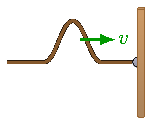
\includegraphics[width=\textwidth]{../figs/waves_reflection_transmission-1.pdf}
        \end{column}
        ~
        \begin{column}{0.45\textwidth}
            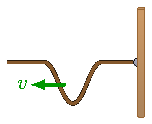
\includegraphics[width=\textwidth]{../figs/waves_reflection_transmission-2.pdf}
        \end{column}
    \end{columns}

\end{frame}

\begin{frame}{Condiciones de borde: Un extremo fijo}

    Si la onda se representa por una función $y \left(x,t\right)$, el hecho de que el extremo permanezca fijo cuando llega el pulso, o la onda, implica que no puede haber desplazamiento vertical de la cuerda, por lo que la expresión matemática adecuada para esta condición de borde es que $$ y \left(0,t\right) = 0. $$ Es importante destacar que esta condición debe cumplirse para cualquier valor de $t$, esto es, el desplazamiento vertical del punto debe ser nulo independientemente del instante en el que la onda llega al extremo fijo.

\end{frame}

\begin{frame}{Condiciones de borde: Un extremo fijo}
    
    Sea $y_1 (x,t) = f(x-v \, t)$ la función que describe el pulso. Si se impone la condición de borde a esta función de onda se obtiene que $$y_1 (0,t) = f(-v \, t) = 0. $$ No es difícil ver que $y_1 (x,t)$ no puede cumplir nunca esta condición ya que, en el mejor de los casos, permite determinan el instante o los instantes de tiempo en los que un punto de la onda pasa por el eje $x$, puesto que $f(-v \, t)$ da la altura del punto de abscisa $x=0$ en función del tiempo, la cual no puede ser nula para todo $t$. Como consecuencia, $y \neq 0$ al menos para ciertos valores de $t$.

    \vs

    Para resolver esta dificultad, podemos observar que después de la reflexión, el pulso se describe como $y_2 \left(x,t\right) = -f \left(x+v \, t\right)$. Esto es, la onda conserva su forma, pero se invierte y se propaga en sentido opuesto al que tenía antes de llegar al extremo fijo, tal como se indicó anteriormente.

\end{frame}

\begin{frame}{Condiciones de borde: Un extremo fijo}   
    
    En consecuencia, podemos pensar que la cuerda es nuevamente infinita y que ambos pulsos se propagan simultáneamente por esta de forma tal que se encuentran en $x=0$. La interpretación física de este modelo consiste en considerar como \emph{reales} a los pulsos que se propagan para los $x < 0$ y \emph{virtuales} aquellos que se propagan sobre los $x>0$. Así, en virtud del principio de superposición, la onda real viene descrita por: $$ y \left(x,t\right) = y_1 \left(x,t\right) + y_2 \left(x,t\right) = f(x-v \, t) -f \left(x+v \, t\right), $$ y observamos el comportamiento de $y \left(x,t\right)$ para los $x<0$.

    \vs

    Si ahora imponemos la condición del extremo fijo: $$ y \left(0,t\right) = f(-v \, t) - f \left(v \, t\right) = 0, $$ podemos ver fácilmente que esta se cumple si $f$ es una función par del tiempo. En consecuencia, es posible satisfacer la condición de borde haciendo uso del principio de superposición.

\end{frame}

\begin{frame}{Condiciones de borde: Un extremo fijo}   

    Vamos a considerar el caso de una onda armónica que se propaga desde $-\infty$ a $0$. Su expresión matemática es entonces: $$ y_1 (x,t) = A \sen \left(\omega \, t - k \, x\right). $$ Para cumplir con la condición de borde correspondiente al extremo fijo, debemos incluir otra onda armónica invertida y que se propague desde $+\infty$ a $0$, por lo que deberá estar dada por: $$ y_2 (x,t) = - \, A \sen \left(\omega \, t + k \, x\right). $$ En virtud de la discusión anterior, la condición de borde debería satisfacerse para la superposición de estas dos ondas: $$ y \left(x,t\right) = y_1 \left(x,t\right) + y_2 \left(x,t\right) = A \left[\sen \left(\omega \, t - k \, x\right) - \sen \left(\omega \, t + k \, x\right)\right] $$

\end{frame}

\begin{frame}{Condiciones de borde: Un extremo fijo}

    Utilizando el teorema del seno de una suma o diferencia de ángulos se obtiene: $$ y \left(x,t\right) = - \, 2 \, A \sen \left(k \, x\right) \cos \left(\omega \, t\right). $$ Como puede verse fácilmente, $y \left(x,t\right)$ satisface la condición de borde para el extremo fijo para todo instante $t$. Notemos, además, que $y \left(x,t\right) $ es una función par del tiempo. Sin embargo, no es necesario que la función de onda que satisface esta condición de borde sea función par del tiempo. Para ver esto, consideremos la función de onda $$ y_1 \left(x,t\right) = A \cos \left(\omega \, t - k \, x\right) $$ La onda que se propaga en el sentido opuesto e invertida respecto de la anterior es: $$ y_2 = - A \cos \left(\omega \, t + k \, x\right) $$ Al sumarlas, se obtiene $$ y \left(x,t\right) = 2 \, A \sen \left(k \, x\right) \sen \left(\omega \, t\right). $$

\end{frame}

\begin{frame}{Condiciones de borde: Un extremo fijo}

    Como vemos, la función función de onda obtenida es una función impar del tiempo. Sin embargo, también satisface la condición de borde. 
    
    \vs 
    
    En conclusión, toda función de onda que es función par del tiempo satisface la condición de borde correspondiente al extremo fijo, pero no toda función de onda que es función impar del tiempo viola dicha condición.

\end{frame}

\begin{frame}{Condiciones de borde: Un extremo fijo}

    En los dos casos antes analizados, vemos que gracias al factor $\sen \left(k \, x\right)$ la función de onda satisface la condición de borde del extremo fijo. Sin embargo, podemos observar también que $y \left(x,t\right) = 0 $ para un conjunto discreto e infinito de valores de $x$, es decir $$ k \, x = n \, \pi \qquad \text{ o bien: } \qquad x = \frac{n \, \pi}{k} = \frac{n \, \lambda}{2},$$ donde $n \in \zz $. Es decir, para semienteros de la longitud de onda, la función de onda se anula para todo instante de tiempo.

    \vs

    Estos valores de $x$, para los que $ y \left(x,t\right) = 0$, se conocen como \emph{nodos}. 

\end{frame}

\begin{frame}{Condiciones de borde: Un extremo libre}

    Consideremos ahora el caso en que tenemos una cuerda semiinfinita que, al igual que en el caso anterior, se extiende desde $-\infty$ hasta $0$, pero que ahora el extremo en $x = 0$ está libre, es decir, que este extremo puede moverse libremente sobre el eje $y$. 
    
    \vs 
    
    Cuando un pulso que se propaga hacia la derecha llega hasta $x = 0$, en cierto instante el extremo libre alcanza su desplazamiento máximo (hacia arriba o hacia abajo). 
    
    \vs 
    
    En ese instante, la componente vertical de la fuerza que la cuerda ejerce sobre el extremo se anula, pero como el elemento que se encuentra inmediatamente a la izquierda ejerce una fuerza que tiende a devolver al extremo a la posición de equilibrio, este último empieza a moverse hacia $y = 0$. 
    
\end{frame}

\begin{frame}{Condiciones de borde: Un extremo libre}
    
    El resultado es la reflexión de la onda conservando su forma pero desplazándose ahora hacia $-\infty$, tal como se muestra en la siguiente figura:

    \begin{columns}
        \begin{column}{0.45\textwidth}
            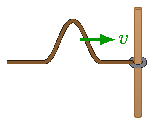
\includegraphics[width=\textwidth]{../figs/waves_reflection_transmission-3.pdf}
        \end{column}
        ~
        \begin{column}{0.45\textwidth}
            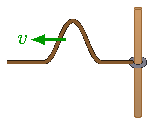
\includegraphics[width=\textwidth]{../figs/waves_reflection_transmission-4.pdf}
        \end{column}
    \end{columns}
    
\end{frame}

\begin{frame}{Condiciones de borde: Un extremo libre}

    Tal como señalamos anteriormente, cuando el extremo libre alcanza su desplazamiento vertical máximo, la componente vertical de la fuerza se anula. Recordemos que dicha componente viene dada por: $$ F_y = F_x \, \pdiff{y}{x}. $$ Por lo tanto, la condición de borde adecuada para el caso de un extremo libre en $x= 0$ es: $$ \pdiff{y \left(0,t\right)}{x} = 0. $$ En virtud de la discusión anterior, esta condición puede satisfacerse con una onda que se propaga desde $+\infty$ hacia $x = 0$. Si $y_1 \left(x,t\right) = f \left(x - v \, t\right)$ es la onda que incide desde la izquierda, la onda que se refleja debe venir dada por $$ y_2 \left(x,t\right) = f \left(x + v \, t\right) $$
    
\end{frame}

\begin{frame}{Condiciones de borde: Un extremo libre}

    Luego, en virtud del principio de superposición, la función de onda que satisface la condición del borde libre es: $$ y \left(x,t\right) = y_1 \left(x,t\right) + y_2 \left(x,t \right)= f \left(x - v \, t\right) + f \left(x + v \, t\right). $$ En este caso, la condición de borde es: $$ \pdiff{y \left(0,t\right)}{x} = \pdiff{f \left(-v \, t\right)}{x} + \pdiff{f \left(v \, t\right)}{x}. $$ La notación aquí utilizada implica que es la derivada la que se evalúa en $x=0$. Se puede ver aquí que si \emph{la derivada} es una función \emph{impar} del tiempo, entonces la condición de borde se satisface, aunque esta \emph{no} es una condición necesaria.
    
\end{frame}

\begin{frame}{Condiciones de borde: Un extremo libre}

    Vamos a considerar nuevamente el caso de una onda armónica. La onda incidente viene dada por: $$ y_1 \left(x,t\right) = A \sen \left(\omega \, t - k \, x\right), $$ esto es, la onda se propaga desde $-\infty$ a $0$. En virtud de la discusión anterior, la correspondiente onda que se propaga en el sentido opuesto debe entonces ser: $$ y_2 \left(x,t\right) = A \sen \left(\omega \, t + k \, x\right). $$ Luego, la onda que satisface la condición de borde libre viene dada por la superposición de estas dos ondas: $$ y \left(x,t\right) = y_1 \left(x,t\right) + y_2 \left(x,t\right) = A \left[\sen \left(\omega \, t - k \, x\right) + \sen \left(\omega \, t + k \, x\right)\right]. $$ Utilizando una vez más el teorema del seno de la suma y diferencia de ángulos se obtiene: $$ y \left(x,t\right) = 2 \, A \cos \left(k \, x\right) \sen \left(\omega \, t\right). $$
    
\end{frame}

\begin{frame}{Condiciones de borde: Un extremo libre}

    No es difícil corroborar que $ y \left(x,t\right) $ satisface la condición de borde correspondiente al extremo libre, puesto que: $$ \pdiff{y \left(x,t\right)}{x} = - 2 \, A \sen \left(k \, x\right) \sen \left(\omega \, t\right).  $$ Es decir que: $$ \pdiff{y \left(0,t\right)}{x} = 0. $$ 
        
\end{frame}

\begin{frame}{Condiciones de borde: Un extremo libre}

    Al igual que en el caso anterior, puede verse que existen infinitos puntos para los cuales $$ \pdiff{y \left(x,t\right)}{x} = 0. $$ Estos valores de $x$ se obtienen de: $$ \sen \left(k \, x\right) = 0, $$ lo cual ocure cuando $ k \, x = n \, \pi $ es decir $$ x = \frac{n \, \pi}{k}, $$ donde $n \in \zz $. En estos valores de $x$ se hallan los puntos donde $ y \left(x,t\right) $ tiene un extremo, por lo que se conocen como \emph{antinodos}.
        
\end{frame}

\begin{frame}{Condiciones de borde: Un extremo libre}

    Los nodos de la función de onda para este caso se hallan planteando: $$ y \left(x,t\right) = 0, $$ es decir: $$ \cos \left(k \, x\right) = 0, $$ lo cual se cumple para: $$ k \, x = \frac{\pi}{2} + n \, \pi = \frac{\pi}{2} \left( 2 \, n + 1\right), $$ donde $n \in \zz $.

\end{frame}

\begin{frame}{Ondas estacionarias: dos extremos fijos}

    Un caso muy interesante de estudio es el de una cuerda de longitud finita $L$ cuyos extremos están fijos. Un ejemplo cotidiano es el de las cuerdas de una guitarra o un violín.

    \vs 

    En este caso, es evidente que ahora vamos a tener dos condiciones de contornos, una para cada extremo, esto es: $$ y \left(0,t\right) = y \left(L,t\right) = 0. $$ Sabemos que la primera de estas dos condiciones se cumple cuando la función de onda viene dada por: $$ y \left(x,t\right) = - \, 2 \, A \sen \left(k \, x\right) \cos \left(\omega \, t\right). $$ 
 
\end{frame}

\begin{frame}{Ondas estacionarias: dos extremos fijos}   
    
    Si ahora se impone la condición para el otro extremo, se obtiene: $$ y \left(L,t\right) = - \, 2 \, A \sen \left(k \, L\right) \cos \left(\omega \, t\right) = 0. $$ Si esta condición ha de satisfacerse para todo instante de tiempo, entonces se debe cumplir necesariamente que: $$ \sen \left(k \, L\right) = 0, $$ lo cual se satisface cuando $ k \, L = n \, \pi $, con $ n \in \zz $ (en principio). Es decir: $$ k_n = \frac{n \, \pi}{L} $$  Ahora bien, recordemos que el número de onda está relacionado con la longitud de onda mediante $$ k = \frac{2 \, \pi}{\lambda}, $$ por lo tanto: $$ \lambda_n = \frac{2 \, L}{n}. $$
    
\end{frame}

\begin{frame}{Ondas estacionarias: dos extremos fijos}

   A su vez, estas están relaciondas con la frecuencia angular ($\omega$) y la frecuencia lineal ($f$) a traves de: $$ k = \frac{\omega}{v} \qquad \text{y} \qquad v = \lambda \, f, $$ donde $v$ es la velocidad de propagación. En consecuencia, se tiene que: $$ f_n = n \left(\frac{v}{2 \, L}\right) \qquad \text{ y } \qquad \omega_n = n \left(\frac{\pi \, v}{L}\right). $$ Hay varios aspectos que es necesario destacar a partir de estos resultados. El primero y el más importante de ellos, es que por una cuerda de longitud finita \emph{no} pueden propagarse ondas de cualquier frecuencia. En otras palabras, solamente ondas de frecuencias bien determinadas pueden satisfacer las condiciones de borde en los dos extremos fijos. Esto se aprecia fácilmente observando que la frecuencia, la longitud de onda y el número de onda dependen de valores fijos, como la longitud de la cuerda ($L$) y la velocidad de propagación $\left(v = \sqrt{\frac{F_x}{\rho \, A}}\right)$. Es por este motivo que estas magnitudes se etiquetan con el subíndice $n$.
    
\end{frame}

\begin{frame}{Ondas estacionarias: dos extremos fijos}

    En segundo lugar, es que si bien las condiciones de borde se satisfacen para cualquier entero $n$, podemos observar que las expresiones de $k_n$, $\lambda_n$, $\omega_n$ y $f_n$ tienen sentido solamente para $n \in \nn $, es decir, $n = 1, 2, 3, \ldots$.

    \vs 

    Para el caso de las frecuencias lineales, vemos que cada una de ellas es un múltiplo de una frecuencia que podemos llamar \emph{fundamental}: $$ f_n = n \, f_1, \text{ donde } f_1 = \frac{v}{2 \, L}. $$ Las frecuencias correspondientes a los $n > 1$ se conocen como \emph{armónicos}, por lo que $n=2$ es el primer armónico, $n=3$ es el segundo armónico, etc.
    
\end{frame}

\begin{frame}{Ondas estacionarias: dos extremos fijos}

    Por último, pero no por eso menos importante, se observa que cada valor de $n$ corresponde a un \emph{modo} de oscilación particular con su propia frecuencia. En la figura siguiente se aprecian los primeros modos.

    \vs

    \begin{columns}
        \begin{column}{0.45\textwidth}
            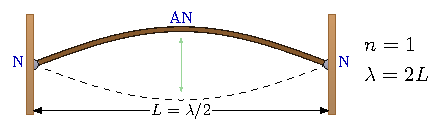
\includegraphics[width=1.\textwidth]{../figs/waves_standing-3.pdf} \\
            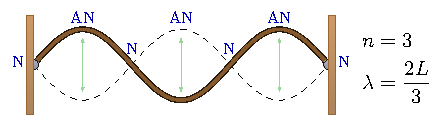
\includegraphics[width=1.\textwidth]{../figs/waves_standing-5.pdf}
        \end{column}
        ~
        \begin{column}{0.45\textwidth}
            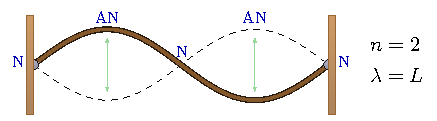
\includegraphics[width=1.\textwidth]{../figs/waves_standing-4.pdf} \\
            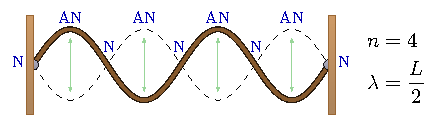
\includegraphics[width=1.\textwidth]{../figs/waves_standing-6.pdf}
        \end{column}
    \end{columns}

\end{frame}

\begin{frame}{Ondas estacionarias: un extremo fijo y otro libre}

    Otro caso interesante es el de una cuerda que tiene un extremo fijo y otro libre. Si suponemos en el extremo fijo está en $x=0$ y el extremo libre en $x=L$, entonces las condiciones de borde serán: $$ y \left(0,t\right) = 0 \qquad \text{ y } \qquad \pdiff{y \left(L,t\right)}{x} = 0. $$ Podemos usar nuevamente la función de onda que satisface la condición de borde del extremo fijo para plantear la condición del extremo libre: $$ \pdiff{y \left(L,t\right)}{x} = - \, 2 \, A \cos \left(k\, L\right) \cos \left(\omega \, t\right) = 0. $$ Dado que esta condición se debe cumplir para todo instante de tiempo, debe ser: $$ \cos \left(k\, L\right) = 0, $$ de donde se obtiene que: $$ k \, L = \frac{\pi}{2} \left( 2 \, n + 1\right). $$

\end{frame}

\begin{frame}{Ondas estacionarias: un extremo fijo y otro libre}

    Vemos en este caso que el número de onda no puede tomar cualquier valor, en virtud de que $L$ es un número fijo: $$ k_n = \frac{\pi}{2} \frac{\left( 2 \, n + 1\right)}{L}. $$ Lo mismo ocurre con la longitud de onda, la frecuencia lineal y la frecuencia angular: $$ \lambda_n = \frac{4 \, L}{2 \, n + 1}, \qquad \omega_n = \left(2 \, n + 1\right) \frac{\pi \, v}{2 \, L} \qquad \text{y} \qquad f_n = \left(2 \, n + 1\right) \frac{v}{4 \, L}, $$ con $n \in \nn$.

\end{frame}

\begin{frame}{Ondas estacionarias: un extremo fijo y otro libre}

    De nuevo, cada valor de $n$ corresponde a un modo de vibración de la cuerda, caracterizado por una valor específico de la frecuencia.

    \vs 

    \begin{columns}
        \begin{column}{0.45\textwidth}
            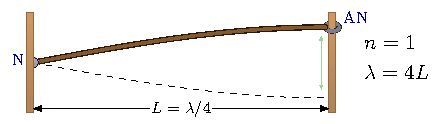
\includegraphics[width=1.\textwidth]{../figs/waves_standing-7.pdf} \\
            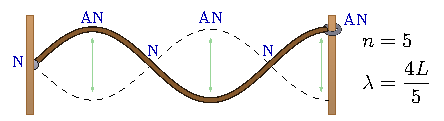
\includegraphics[width=1.\textwidth]{../figs/waves_standing-9.pdf}
        \end{column}
        ~
        \begin{column}{0.45\textwidth}
            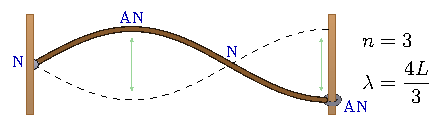
\includegraphics[width=1.\textwidth]{../figs/waves_standing-8.pdf} \\
            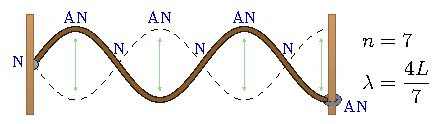
\includegraphics[width=1.\textwidth]{../figs/waves_standing-10.pdf}
        \end{column}
    \end{columns}

\end{frame}

\begin{frame}{Solución general de la ecuación de ondas y series de Fourier}

    Como conclusión de lo discutido anteriormente, se observa que hay una solución de la ecuación de ondas para cada valor de $n$, esto es: $$ y_n \left(x,t\right) = - \, 2 \, A \sen \left(k_n \, x\right) \cos \left(\omega_n \, t\right) $$ Ahora bien, en virtud del principio de superposición, la suma de todas estas (infinitas) soluciones es también solución: $$ y \left(x,t\right) = \sum_{n=1}^{\infty} \left[- \, 2 \, A \sen \left(k_n \, x\right) \cos \left(\omega_n \, t\right)\right]. $$ Como la función de onda puede ser cualquier función $y \left(x,t\right) = f \left(x - v \, t\right)$, la expresión anterior indica que toda solución puede expandirse en senos y cosenos, esto se conoce como expansión en series de Fourier.

\end{frame}

\begin{frame}{Solución general de la ecuación de ondas y series de Fourier}

    Por otro lado, vemos que la solución queda expresada como el producto entre una función que depende solamente de $x$ y otra que depende solamente del tiempo. Esto inspira la idea de que para resolver la ecuación de ondas clásica, se puede proponer una función que tenga estas características, es decir: $$ y \left(x,t\right) = f(x) \, g(t),$$ con la prescripción de que $g (0) = 1$ de forma tal que $y\left(x,0\right) = f(x)$ represente la forma inicial de la cuerda.

\end{frame}

\section{Reflexión y transmisión de ondas en discontinuidades}

\begin{frame}{Reflexión y transmisión de ondas en discontinuidades}

    Vamos a aprovechar nuestro conocimiento sobre las condiciones de contorno para estudiar lo que ocurre cuando una onda se encuentra con una discontinuidad en el medio en el que se está propagando. Esto ocurre cuando, por ejemplo, una onda llega al punto en que la cuerda en que se estaba propagando se une con otra cuerda que tiene una densidad y tensión diferentes.

\end{frame}

\end{document}

\begin{frame}{}



\end{frame}